
\part{Discrete replicator and random walk}
\noindent \begin{flushright}
\textit{The theory of evolution is based on the }\\
\textit{struggle for life and the survival of the fittest. }\\
\textit{Yet cooperation is common between members of the same }\\
\textit{species and even between members of different species.}\\
\textit{ }Robert Axelrod
\par\end{flushright}

In this chapter, we propose a spatial discrete replicator equation.
We suppose the players as random walkers on a square lattice with
a sort of drift term due to the discrete replicator equation \cite{hofbauer_evolutionary_1998}:
\[
p_{\ell}^{k+1}=p_{\ell}^{k}\frac{c+\mathbf{e}_{\ell}^{T}A\mathbf{p}}{c+\mathbf{p}^{T}A\mathbf{p}}
\]
here c is a positive constant corresponding to the fitness in the
absence of interaction, $p_{\ell}^{k}$ is the frequency of strategy
$\ell$ at time $k$, and as in \ref{eq:replicator}, $\mathbf{e}_{\ell}^{T}A\mathbf{p}$
is the payoff of the focal player playing the strategy $\ell$ against
the population playing the mixed strategy $\mathbf{p}$, and $\mathbf{p}^{T}A\,\mathbf{p}$
is the payoff of the focal player playing the same mixed strategy
$\mathbf{p}$ of the population. Finally, we simulate it and discuss
the relation with the previous PDEs.

\section{A heuristic derivation\label{sec:A-heuristic-derivation} }

Consider a population of agents distributed on the cubic lattice $\mathbb{Z}^{m}$
and let $N^{k}=N^{k}\left(x\right)$ be the number (density) of agents
at site $x\in\mathbb{Z}^{m}$ at the time step $k$. Let $n_{\ell}^{k}\left(x\right)$
be the number of agents at $x$ playing strategy $\ell$ at time $k$,
so that, for games with two strategies, $\ell=1,2$ and $\sum_{\ell}n_{\ell}^{k}\left(x\right)=N^{k}\left(x\right)$.

Let $U\left(x\right)\subset\mathbb{Z}^{m}$ be the set of first neighbours
of $x$, i.e., $U\left(x\right)=\left\{ y\in\mathbb{Z}^{m}:\exists i\,\mid\,y_{i}=x_{i}\pm1\text{ and }y_{j}=x_{j}\text{ otherwise}\right\} $,
and define a random walk on the lattice by assigning uniform probability
to the jump from a point to each of its neighbours, i.e.:
\[
\mathbb{P}\left(y|x\right)=\begin{cases}
\frac{1}{2m} & \text{ if }y\in U(x)\\
0 & \text{otherwise}.
\end{cases}
\]
Here, we assume that two processes are active at each time step $k$
and lattice point $x$, and for every strategy $\ell$: 
\begin{itemize}
\item First, the population $n_{\ell}^{k}\left(x\right)$ of $\ell$-players
at each lattice point reproduces according to a discrete replicator
dynamics: the rate of growth of a subpopulation that plays $\ell$
is just its relative fitness, i.e. the ratio between the payoff of
the pure strategy against the population, and the average payoff of
the population. The number of offspring is therefore: 
\[
n_{\ell}^{k}\left(x\right)\frac{c+\frac{{\bf e}_{\ell}\cdot A{\bf n}^{k}\left(x\right)}{N^{k}\left(x\right)}}{c+\frac{{\bf n}^{k}\left(x\right)\cdot A{\bf n}^{k}\left(x\right)}{\left(N^{k}\left(x\right)\right)^{2}}},
\]
where, for two strategies, ${\bf n}^{k}\left(x\right)=\left(n_{1}^{k}\left(x\right),n_{2}^{k}\left(x\right)\right)$.
\item Then, the offspring remain at site $x$, but the parent population
migrates to the neighbouring lattice points according to the random
walk above. Hence, since the probability of remaining at the site
vanishes, the expected number of parents at site $x$ at time $k+1$
is given by:
\[
-n_{\ell}^{k}(x)+\sum_{y\in U(x)}\mathbb{P}\left(y|x\right)n_{\ell}^{k}\left(y\right)=\frac{1}{2m}\left(\sum_{y\in U(x)}\mathbb{P}\left(y|x\right)n_{\ell}^{k}\left(y\right)-2m\,n_{\ell}^{k}\left(x\right)\right),
\]
that accounts for the migration to site $x$ from its neighbours.
\end{itemize}
Hence, the population of $\ell$-agents at time $k+1$ at $x$ is:
\[
n_{\ell}^{k+1}(x)=\frac{1}{2m}\left(\sum_{y\in U(x)}\mathbb{P}\left(y|x\right)n_{\ell}^{k}\left(y\right)-2m\,n_{\ell}^{k}\left(x\right)\right)+n_{\ell}^{k}\left(x\right)\frac{c+\frac{{\bf e}_{\ell}\cdot A{\bf n}^{k}\left(x\right)}{N^{k}\left(x\right)}}{c+\frac{{\bf n}^{k}\left(x\right)\cdot A{\bf n}^{k}\left(x\right)}{\left(N^{k}\left(x\right)\right)^{2}}},
\]
which is our basic update rule for the population.

Introducing the Laplacian operator of the lattice by: 
\[
\mathcal{L}=B-2mI,
\]
where $I$ is the $K\times K$ identity matrix, $K$ is the number
of sites of the portion of the lattice we are working on, and $B$
is the adjacency matrix of the lattice, such that $B_{xy}=1$ only
if $y\in U(x)$, and zero otherwise, we can rewrite the update rule
as in terms of the Laplacian: 
\begin{equation}
n_{\ell}^{k+1}(x)=\frac{1}{2m}\sum_{y\in U(x)}\mathcal{L}_{xy}n_{\ell}^{k}\left(y\right)+n_{\ell}^{k}\left(x\right)\frac{c+\frac{{\bf e}_{\ell}\cdot A{\bf n}^{k}\left(x\right)}{N^{k}\left(x\right)}}{c+\frac{{\bf n}^{k}\left(x\right)\cdot A{\bf n}^{k}\left(x\right)}{\left(N^{k}\left(x\right)\right)^{2}}}.\label{eq:discr}
\end{equation}
For instance, in case of a 1-dimensional lattice, letting $x=i\in\mathbb{Z}$,
we have:
\[
n_{\ell}^{k+1}(i)=\frac{1}{2}(n_{\ell}^{k}(i+1)-2n_{\ell}^{k}(i)+n_{\ell}^{k}(i-1))+n_{\ell}^{k}(i)\frac{c+\frac{{\bf e}_{\ell}\cdot A{\bf n}^{k}(i)}{N^{k}(i)}}{c+\frac{{\bf n}^{k}\left(i\right)\cdot A{\bf n}^{k}(i)}{(N^{k}(i))^{2}}}.
\]


\section{The simulations\label{sec:The-simulations-1}}

We will study the dynamics \ref{eq:discr} on a two dimensional plane
$\left[0,L_{x}\right]\times\left[0,L_{y}\right]$ in a time interval
$\left[0,T\right]$, i.e. the equation for a two dimensional lattice
$x\equiv\left(i,j\right)\in\mathbb{Z}^{2}$ is:
\begin{align*}
n_{\ell}^{k+1}\left(i,j\right) & =\frac{1}{4}\left[\left(n_{\ell}^{k}\left(i+1,j\right)-2n_{\ell}^{k}\left(i,j\right)+n_{\ell}^{k}\left(i-1,j\right)\right)\right.\\
 & +\left.\left(n_{\ell}^{k}\left(i,j+1\right)-2n_{\ell}^{k}\left(i,j\right)+n_{\ell}^{k}\left(i,j-1\right)\right)\right]\\
 & +n_{\ell}^{k}(i,j)\frac{c+\frac{{\bf e}_{\ell}\cdot A{\bf n}^{k}(i,j)}{N^{k}(i,j)}}{c+\frac{{\bf n}^{k}\left(i,j\right)\cdot A{\bf n}^{k}(i,j)}{(N^{k}(i,j))^{2}}}
\end{align*}
Since it is discrete, performing simulations is much simpler. Then,
as done in the previous part, we consider three forms of $n_{1}^{0}\left(i,j\right)$
and $n_{2}^{0}\left(i,j\right)$:
\begin{enumerate}
\item a random value between $0$ to $1$, i.e. for $\ell=1,2$:
\[
\forall x,y\quad n_{\ell}^{0}\left(i,j\right)=random\left[0,1\right];
\]
\item a single defector in a sea of cooperators, i.e. for the cooperators:
\[
n_{1}^{0}\left(i,j\right)=\begin{cases}
1 & if\ i\neq\frac{L_{x}}{2}\ or\ j\neq\frac{L_{y}}{2}\\
0 & otherwise
\end{cases}
\]
 and for the defectors:
\[
n_{2}^{0}\left(i,j\right)=\begin{cases}
1 & if\ i=\frac{L_{x}}{2}\ and\ j=\frac{L_{y}}{2}\\
0 & otherwise
\end{cases};
\]
\item a delta-type of defectors surrounded by cooperators, i.e.:
\begin{align*}
n_{1}^{0}\left(i,j\right) & =\begin{cases}
1 & if\ i\neq\frac{L_{x}}{2}\\
0 & otherwise
\end{cases}\\
n_{2}^{0}\left(i,j\right) & =\begin{cases}
1 & if\ i=\frac{L_{x}}{2}\\
0 & otherwise
\end{cases}
\end{align*}
\end{enumerate}
We choose zero value boundary conditions, i.e. for $\ell=1,2$:
\[
n_{\ell}^{k}\left(0,0\right)=n_{\ell}^{k}\left(0,L_{y},t\right)=n_{\ell}^{k}\left(L_{x},0,t\right)=n_{\ell}^{k}\left(L_{x},L_{y},t\right)=0\quad\forall t\in\left[0,T\right].
\]


\subsection{Random initial condition}

We set a random initial position of cooperators and defectors in equal
proportion (fig \ref{fig:rand-1}). 

\begin{figure}
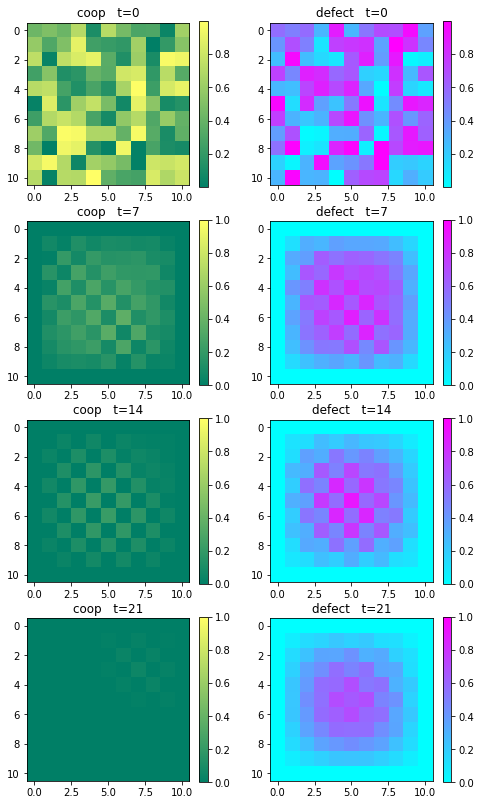
\includegraphics[width=0.75\textwidth]{immagini/discr-rand}

\caption{\label{fig:rand-1}Numerical solution of $n_{1}$ and $n_{2}$ in
$T=21$ and $L_{x}=L_{y}=10$ of \ref{eq:discr}. We set $b=1.85$.}
\end{figure}


\subsection{One defector in a sea of cooperators}

Secondly, we study the dynamics of the two population setting at the
starting time the defectors in a single central point surrounded by
the cooperators (fig \ref{fig:onedef-1}). 

\begin{figure}
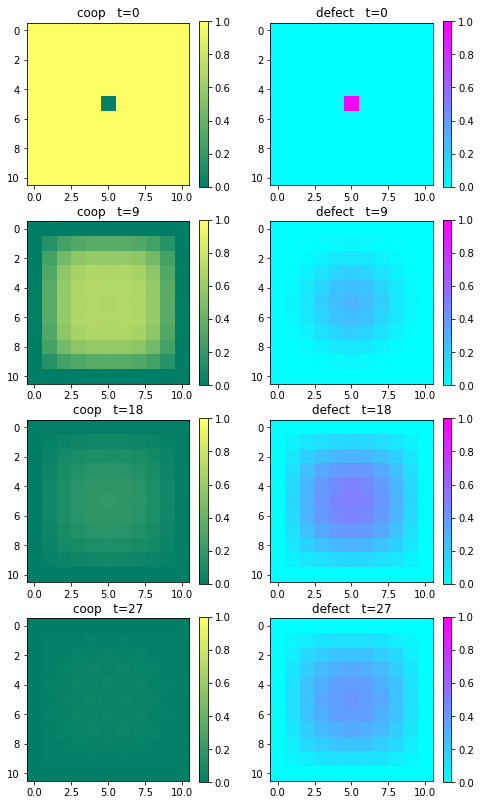
\includegraphics[width=0.75\textwidth]{immagini/discr-onedef}

\caption{\label{fig:onedef-1}Numerical solution of $n_{1}$ and $n_{2}$ in
$T=27$ and $L_{x}=L_{y}=10$ of \ref{eq:discr}. We set $b=1.85$.}
\end{figure}


\subsection{Delta initial condition}

Finally, we arrange the defectors in the delta-type function in the
space surrounded by the cooperators, at the initial time. We can see
the evolution below (fig \ref{fig:delta-1}). 

\begin{figure}
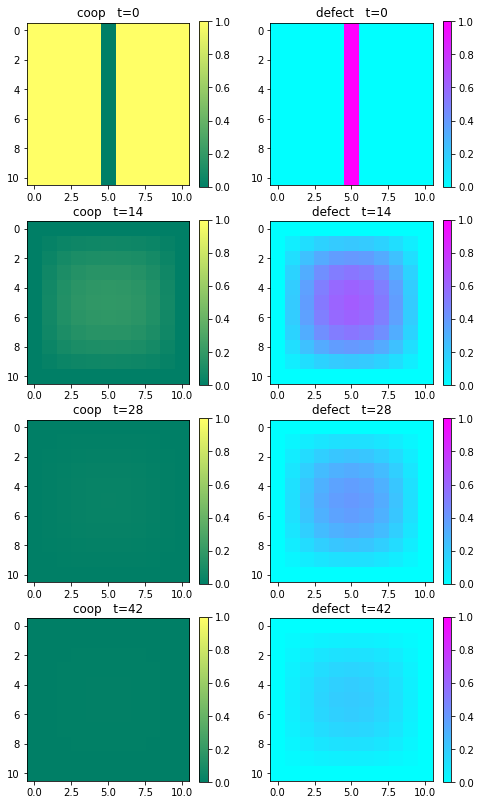
\includegraphics[width=0.75\textwidth]{immagini/discr-delta}

\caption{\label{fig:delta-1}Numerical solution of $n_{1}$ and $n_{2}$ in
$T=42$ and $L_{x}=L_{y}=10$ of \ref{eq:discr}.We set $b=1.85$.}
\end{figure}


\subsection{Phase diagram and conclusion}

The equation \ref{eq:discr} gives similar results to those we have
seen in the continuous models. In figure \ref{fig:N_tot}, we compare
the evolution of the total number $\tilde{N}$ in the three models,
for the 2-dimensional discrete model it is:
\[
\tilde{N}^{k}=\sum_{x\in\mathbb{Z}^{2}}N^{k}\left(x\right)
\]

\begin{figure}

\subfloat[]{

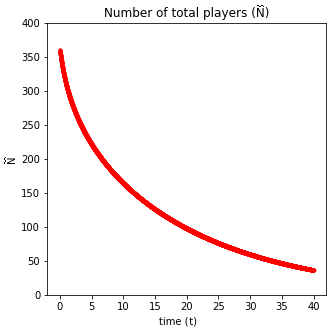
\includegraphics[width=0.33\textwidth]{immagini/Ntot_CN}} \subfloat[]{

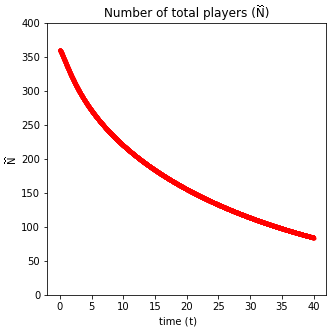
\includegraphics[width=0.33\textwidth]{immagini/Ntot_l-w}}\subfloat[]{

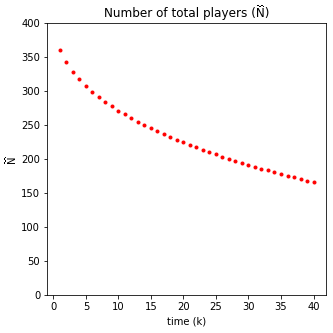
\includegraphics[width=0.33\textwidth]{immagini/Ntot_discr}

}\caption{\label{fig:N_tot} Evolution of the total density $\tilde{N}$ for
$T=40$ in the parabolic model (A), in the hyperbolic model (B) and
in the discrete model (C).}

\end{figure}

We can observe that in the three models $\tilde{N}$ decreases. In
the hyperbolic the speed of decrease is slower than the parabolic
and this is due to the ad-hoc flux, which forces the speed limit,
so there is no new information, but in the discrete one the decrease
is the slowest, with no assumption on the dispersal speed.

Moreover, as done for the continuous model, we want to try to understand
if there is a phase transition in the probability of a strategy varying
$b$. So, calling $\left|V\right|$ the number of nodes in the lattice,
the probability of the $\ell-th$ strategy is:
\[
p_{\ell}=\frac{\frac{1}{\left|V\right|}\sum_{\mathbf{x}:\forall\mathbf{x}\in\Gamma}n_{\ell}(\mathbf{x},t)}{\frac{1}{\left|V\right|}\sum_{j}\sum_{\mathbf{x}:\forall\mathbf{x}\in\Gamma}n_{j}(\mathbf{x},t)}\qquad t\rightarrow+\infty
\]

\begin{figure}
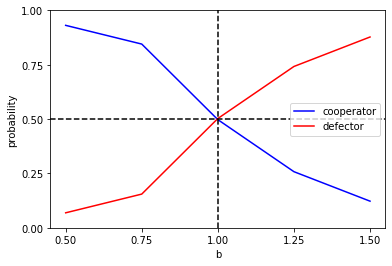
\includegraphics[width=0.75\textwidth]{immagini/discr_phase}\caption{\label{fig:Phase-diagrams}Phase diagrams of the parabolic model (A)
and of the hyperbolic model (B).}
\end{figure}

As for the continuous model, in fig \ref{fig:Phase-diagrams} we observe
a phase transition in $b=1$. This means that we have a phase transition
when the temptation $T$ becomes higher than the reward $R$.
